%this is a document full of really basic LaTex stuff
%most of the information came from here: http://en.wikibooks.org/wiki/LaTeX

\documentclass{article} %there are other document class options but I don't know them yet.
                        %there are also \documentclass[options]{class}
%\usepackage{package1, package2, ...}
\usepackage{graphicx}

%some packages require options and must be listed separately
%\usepackage[options]{package3}

%Here are some useful packages
%\usepage{setspace} -- useful for setting line and character spacing throughout the document
%\usepackage{hyphenat} -- the proper way to hyphenate shit
%\usepackage{microtype}
%\DisableLigatures{encoding = *, family = *} -- use these two together to disable ligatures 

\begin{document} %anything above here is the preamble

\title{A Bunch of \LaTeX{} Stuff} %obviously there's a fancy way to write LaTeX
\author{Nik Hartman\\
        Johns Hopkins} %continue onto another line with \\
\date{April 2014}
\maketitle

\begin{abstract}

In this abstract I will describe nothing at all about the content of this document. It is only here 
so that I can look and see if it is formatted in a pleasing way.

\end{abstract}

%Text formatting

%\being{doublespace} -- similar spacing commands are available
%\end{doublespace}
%\hfill -- pushes any text following toward the right margin
%\vfill -- pushes any text following to the bottom of the page
%\clearpage -- stops all output in float? and starts new page
%\newpage -- starts new page or column (if two columns are being used)

%if using a command many times to change the formatting of certain words, 
%it is best to define a macro for it using \newcommand. This way if you want 
%to format all of those words in some other way later, only one line must be changed.

%there are three types of dashes for compound-words, numbering 16--17, and --- interuptions --- in text
%also elipses \ldots

%\being{verbatim} -- this will recreate every character as it is typed
%\end{verbatim}

\hfill\newline %if you want to create an empty line with \newline or \\ you need to put some shit in it like \hfill
\noindent It is not necessary to put the text in a section, but it does seem that the sections are formatted 
slightly differently than the rest of the text. For example, the first paragraph of a section is not
indented, but the first paragraph of this text is. 

\clearpage %really just to see what happens when I get over two pages.

\section{The First Section} % use \section*{} to suppress numbering
                            % items will be automatically added to table of contents
                            % \section[TOC title]{longer title} can be used as well

Here is some text! Spaces are ignored. I think skipping a line should start a new paragraph. I'm just 
going to put some more crap here so it is clear what's going on.

Is that true? Maybe that behavior is influenced by my choice of document class? Ah. It is a new paragraph.
It's just hard to tell when I don't write more than one line of text.

\subsection{A Subsection} 

This section should have some additional information pertaining to the topic of the First Section.
There might also be some related subsection to follow.

\section{Making a figure with a caption}

The contents of this section should be very straightforward. How do I produce a reference to a figure? 
Like, if I want to talk about Figure~\ref{fig:tour} on page~\pageref{fig:tour}. That Figure was very easy to 
make and worked as a JPG or when converted to EPS. On the other hand, Figure~\ref{fig:sem} on page~\pageref{fig:sem} 
was a pain. When converting to EPS, it seems the 'density' key is important. For the TIFF from the SEM density=72 gave a final image with the same resolution as the original TIFF.

\begin{figure}[h] %[h] puts the figure right here in the text, if possible based on some other criteria.
\centering %optional. it's purpose is obvious.
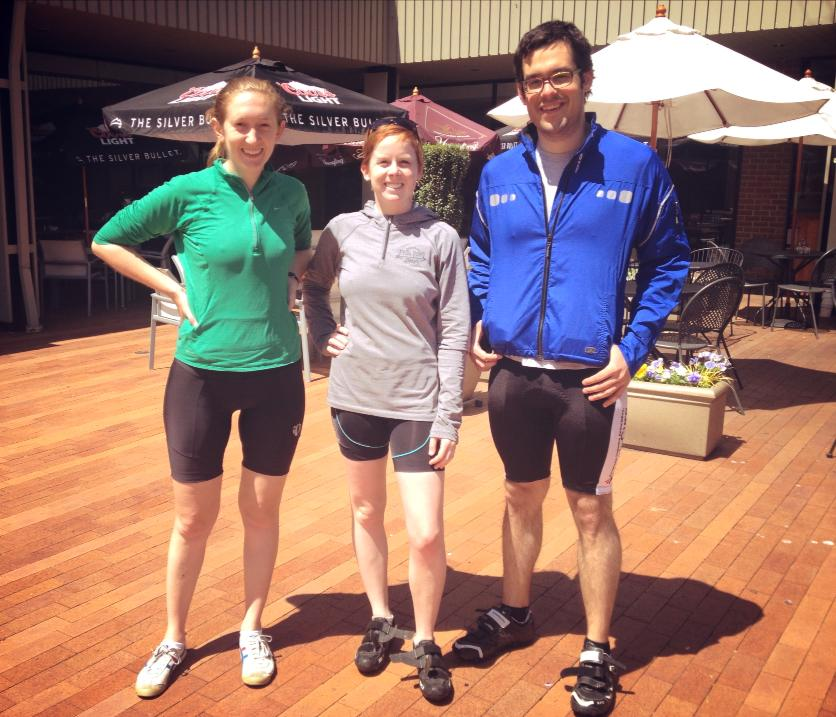
\includegraphics[width = 0.6\textwidth]{tour_training.jpg}
\caption{This color image works as a JPG or when converted to EPS.}
\label{fig:tour}
\end{figure}

Notice how I forced that first image to go right in here?! That worked great for this image, but not for Figure~\ref{fig:sem}.

\begin{figure}
\centering
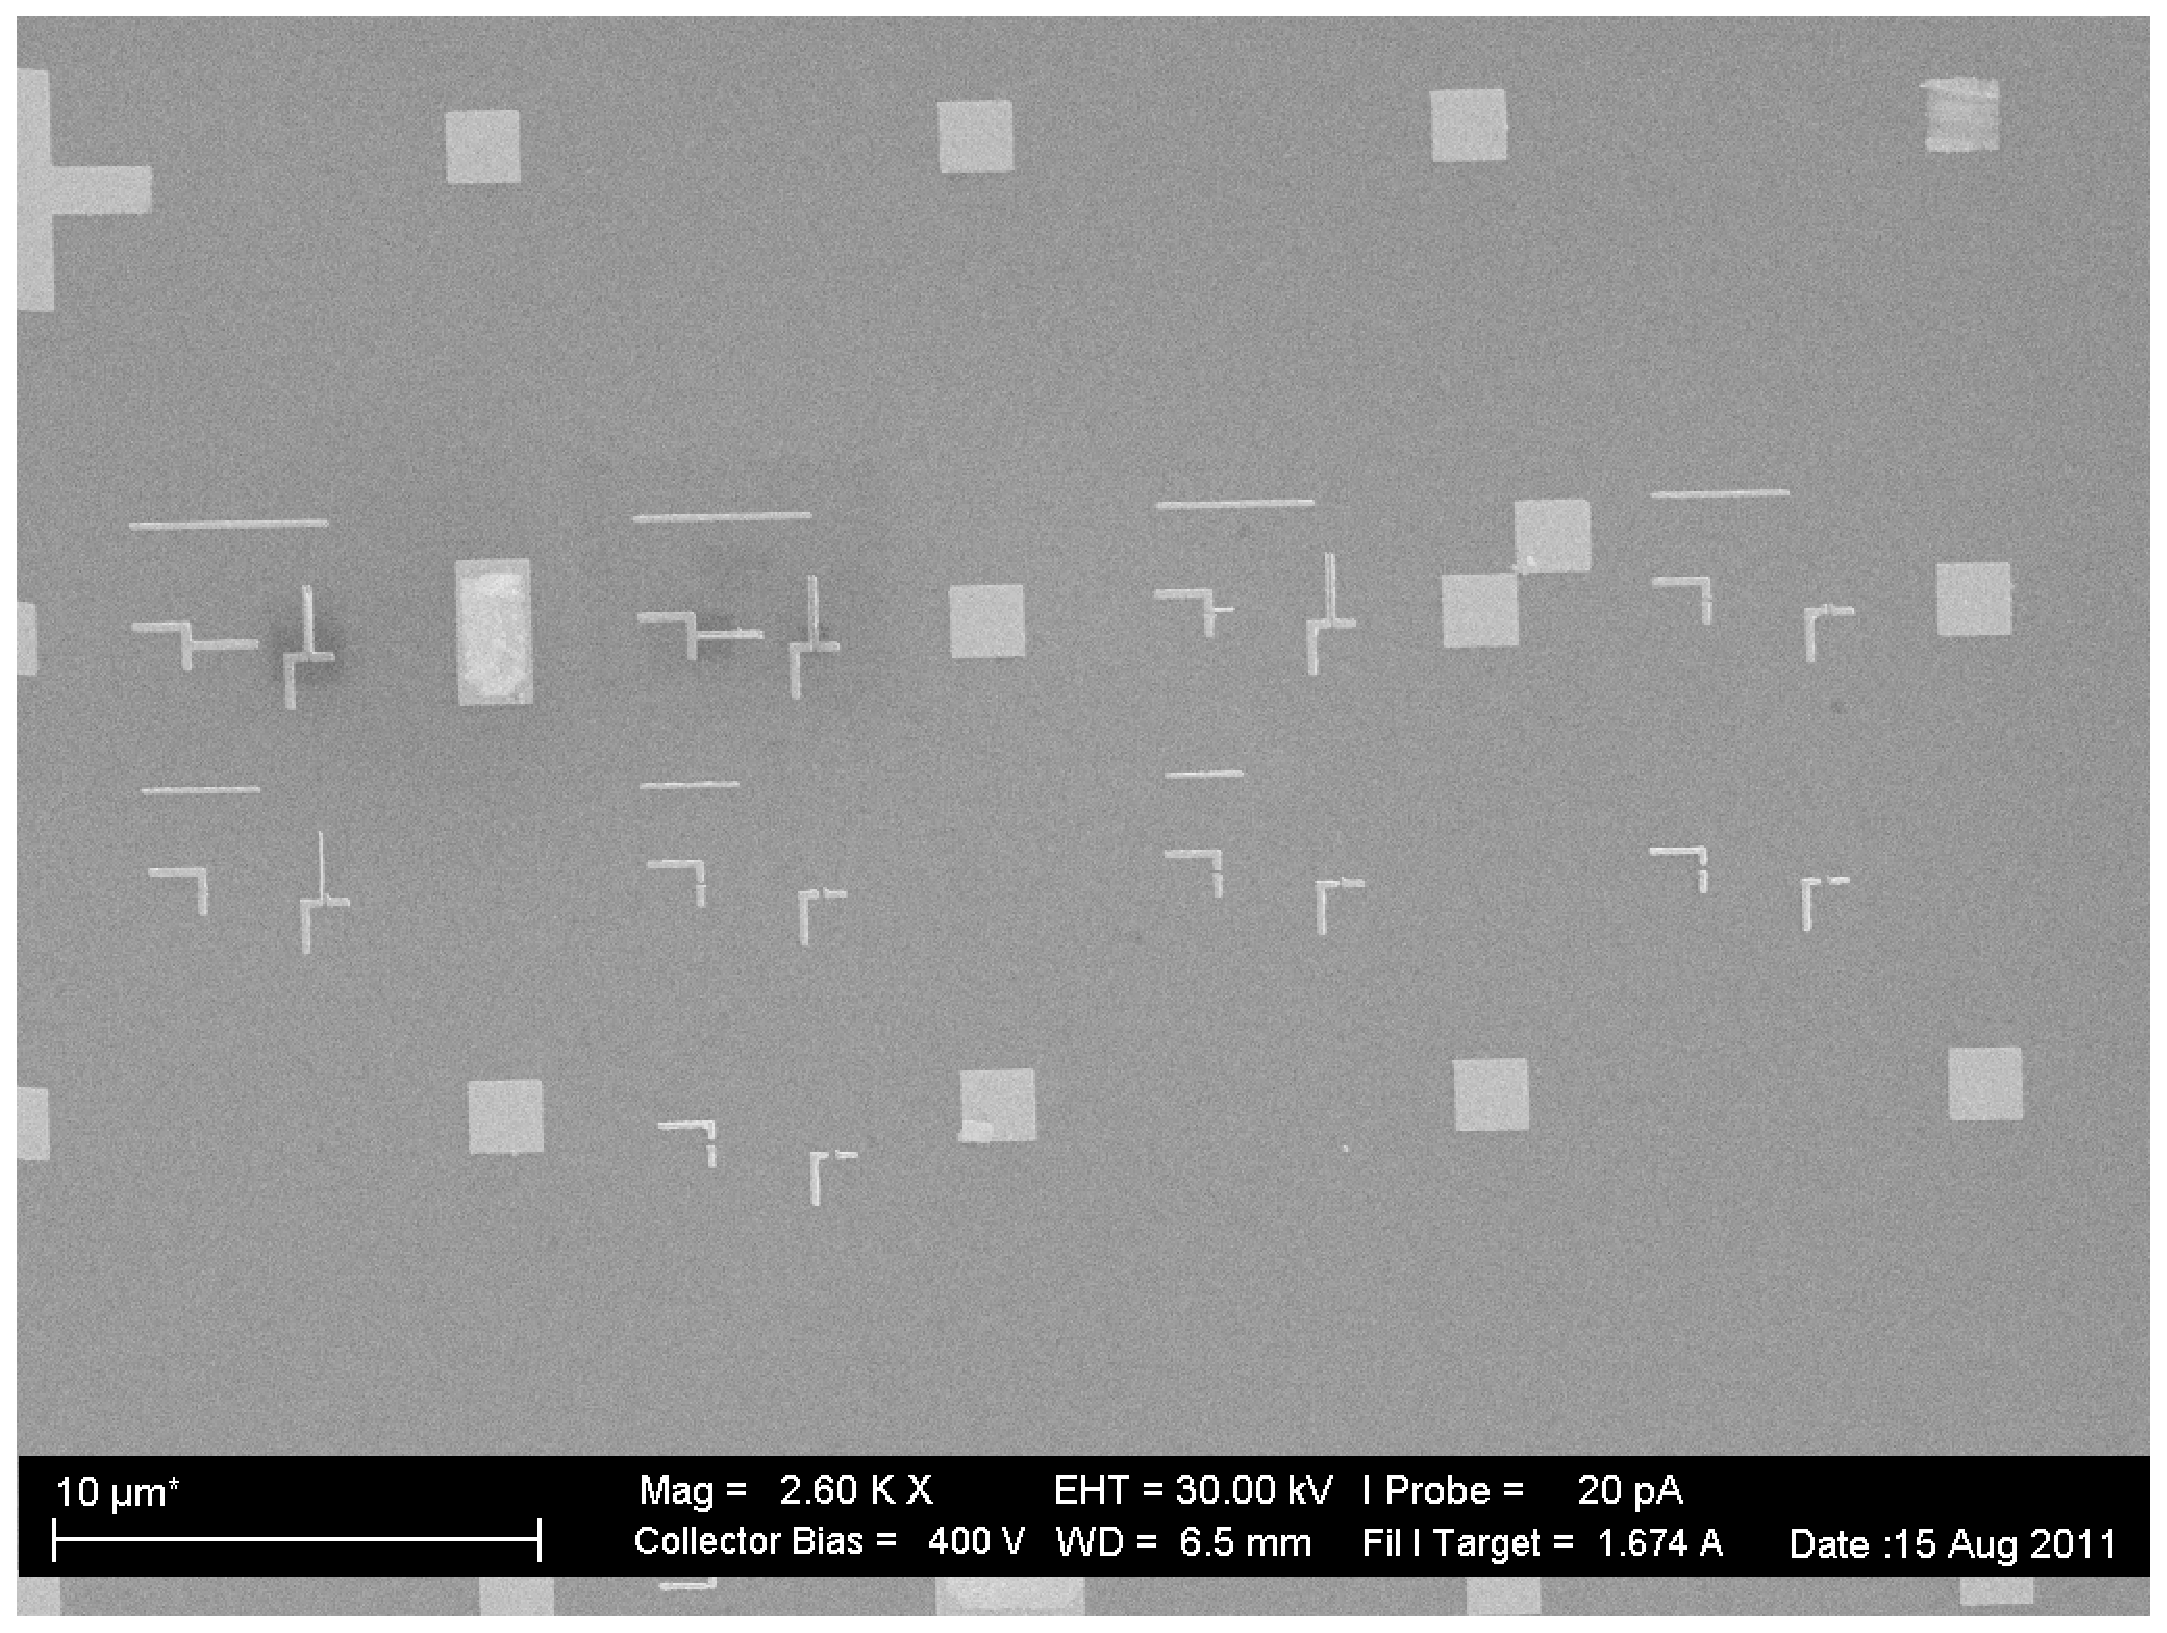
\includegraphics[width = 0.8\textwidth]{testimage.eps}
\caption{This TIFF from the SEM had to first be converted to EPS.}
\label{fig:sem}
\end{figure}

I'm going to write a bunch of stream of consciousness crap right here. What I want to know is, whether or not the image in fig 2 will be pushed around on it's page once my text catches up to the next page. A few more lines should be enough. This is a lot of pointless typing. Certainly, there should be a better way to figure this out. However, the point of this document is to learn to do things the hard way now, so I'm aware of the easy way later. BOOM! That's it. The image now lives on the top of page 3. It looks like there is a package , floats?, for moving these things around the hard way, if the automatic formatting doesn't work.

\section{Making a table}

This section will show some tables full of arbitrary crap. Hopefully, there will be some formatting options illustrated as well.

\begin{center}
    \begin{tabular}{| r | l || p{50mm} |} %also a [pos] option
        \hline %a horizontal line
        This & That & I can write a whole ton of stuff in this paragraph column. Toooooons of stuff here.\\ \hline
        No word wrap here. & Oh shit! & Less stuff here. \\
        \hline
    \end{tabular}
\end{center}

Without using the center environment, things get a little weird.
\hfill \\
\begin{tabular}{| c | c |}
    \hline
    Look & at \\ \hline
    this & shit \\
    \hline
\end{tabular}
The table just gets jammed into that exact location. There is a ton of additional information available on the LaTeX wikibooks pages. Actually, that's true for this entire document. This was basically just me working through that thing.

There are way too many table options to discuss much more. You're going to have to Google your way out of any additional trouble, chief.

\end{document} %anything after this line is ignored